\section{Conception de la charge utile}
\href{https://youtu.be/uHOsxEK5CUA}{Visualiser la Video}


\textbf{Sujet et Charge Utile}

\begin{itemize}
    \item Le \textbf{sujet} et la \textbf{charge utile} sont les principaux moteurs de conception, car ils justifient l'existence de la mission.
    \item Le sujet détermine :
    \begin{itemize}
        \item L'\textbf{emplacement} ou l'\textbf{orbite} que le vaisseau spatial doit atteindre.
        \item La \textbf{charge utile} à intégrer.
        \item Toutes les \textbf{exigences de conception} qui influencent la conception du bus spatial.
    \end{itemize}
    \item Les classifications des charges utiles incluent :
    \begin{itemize}
        \item \textbf{Observation}.
        \item \textbf{Communications ou navigation}.
        \item \textbf{In situ}.
        \item \textbf{Action à distance}.
        \item \textbf{Vols spatiaux habités}.
    \end{itemize}
    \item La majorité des charges utiles des \textbf{CubeSats} concernent :
    \begin{itemize}
        \item L'\textbf{observation de la Terre}.
        \item La \textbf{communication}.
        \item La \textbf{navigation}.
        \item La \textbf{science et la technologie}.
    \end{itemize}
    \item Les charges utiles des vols spatiaux habités et celles d'\textbf{action à distance} sont rarement utilisées sur les CubeSats.
    \item Les charges utiles d'\textbf{observation} sont principalement utilisées pour :
    \begin{itemize}
        \item L'étude de l'\textbf{espace lointain} (\textit{exoplanètes, phénomènes astronomiques, effets du soleil sur la météo spatiale}).
        \item L'étude de la \textbf{Terre} (\textit{climat, surveillance, cartographie de la surface terrestre, plans d'eau}).
    \end{itemize}
    \item Ces charges utiles fonctionnent dans différentes \textbf{bandes de longueurs d'onde}.
\end{itemize}

\begin{figure}[H] % H force l'affichage ici
    \centering
    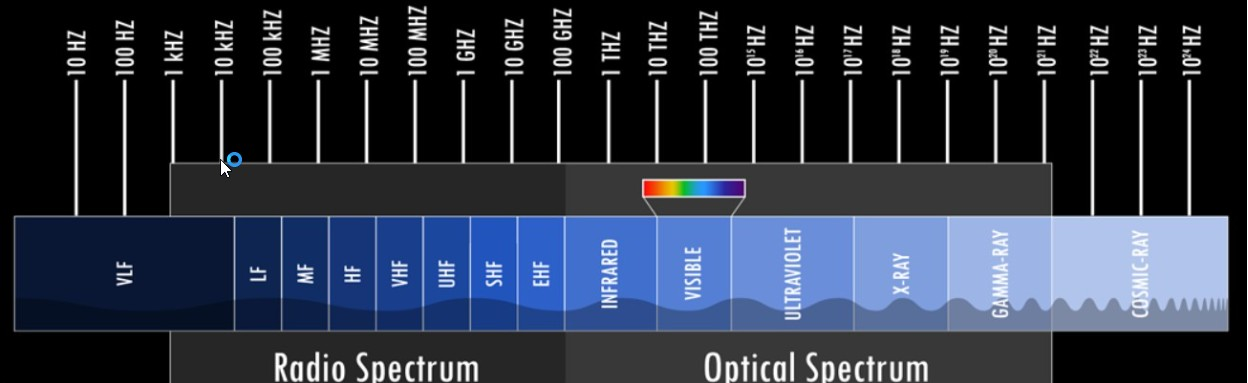
\includegraphics[width=0.8\textwidth]{figures/3.15.jpg}
    \caption{NASA electromagnetic spectrum mapping to space phenomena. Image courtesy of NASA.}
    \label{fig:communication2}
\end{figure}
\textbf{Types de Charges Utiles de Communication et Navigation}
\begin{itemize}
    \item Les charges utiles de \textbf{communication} peuvent être classées en :
    \begin{itemize}
        \item \textbf{Systèmes unidirectionnels} : recueillent des informations sans transmission active.  
        \item \textbf{Systèmes bidirectionnels} : recueillent et transmettent des informations.  
    \end{itemize}
    \item Les charges utiles de \textbf{navigation} suivent et transmettent des informations de position, comme :
    \begin{itemize}
        \item Le \textbf{système de positionnement global} (\textbf{GPS}).  
        \item Les plateformes de \textbf{radio définie par logiciel} (\textbf{SDR}).  
    \end{itemize}
    \item Les charges utiles \textbf{in-situ} mesurent directement les signaux de l’environnement qui ne peuvent pas être détectés à distance, tels que :
    \begin{itemize}
        \item Le \textbf{champ magnétique}.  
        \item La \textbf{gravité}.  
        \item La \textbf{collecte d’échantillons}.  
    \end{itemize}
\end{itemize}
\textbf{Spécificités du Kit Artemis}

\begin{itemize}
    \item Nous nous concentrerons sur les \textbf{charges utiles d'observation}, car le kit Artemis CubeSat est équipé d'une \textbf{caméra visible-IR}.  
    \item L'équipe \textbf{Ke Ao} de l'\textbf{UH Manoa} souhaite prendre une \textbf{photo d’Hawaï} depuis l'orbite terrestre basse et la transmettre aux opérateurs de mission.  
    \item La charge utile est une \textbf{caméra visible} basée sur un \textbf{Raspberry Pi}.  
\end{itemize}
\textbf{Contraintes de la Charge Utile}

Avant de concevoir le sous-système du bus spatial en fonction de la charge utile, il est essentiel d'examiner les contraintes liées à la conception de la charge utile. Il existe quatre types de contraintes :

\begin{itemize}
    \item \textbf{Contraintes fondamentales} :  
    \begin{itemize}
        \item Limite de diffraction.  
        \item Bruit photonique.  
        \item Limite de Nyquist.  
        \item Ces limites sont imposées par les lois de la physique et restreignent l'observation, rendant certaines missions impossibles, même avec des avancées technologiques.  
    \end{itemize}

    \item \textbf{Contraintes technologiques} :  
    \begin{itemize}
        \item Limitations des détecteurs de pointe (taille et performances).  
        \item Forme, précision, fabrication et alignement optiques.  
        \item Vitesse de traitement des données.  
        \item Même en dehors des limites théoriques, les détecteurs et optiques fabriqués auront des performances suboptimales.  
    \end{itemize}

    \item \textbf{Contraintes de mission} :  
    \begin{itemize}
        \item Contraintes de taille, de poids et de puissance (\textbf{SWaP}) dues à la conception du vaisseau spatial et au lanceur sélectionné.  
        \item Certaines charges utiles ne peuvent pas être miniaturisées davantage sans compromettre la performance de la mission.  
    \end{itemize}

    \item \textbf{Contraintes programmatiques} :  
    \begin{itemize}
        \item Coût.  
        \item Planning et délais.  
        \item Risques et exigences réglementaires.  
        \item Ces contraintes peuvent empêcher une mission réalisable sur le plan scientifique et technologique d’être menée à bien.  
    \end{itemize}
\end{itemize}

Cette séquence de contraintes évolue du niveau scientifique le plus élevé jusqu'aux réalités physiques et sociétales des missions spatiales.

\textbf{Spécificités du Kit Artemis}
\begin{itemize}
    \item Pour le projet \textbf{Ke Ao}, la charge utile n'est pas une technologie de pointe passée.  
    \item La caméra \textbf{Raspberry Pi} est une technologie éprouvée.  
    \item Ses caractéristiques physiques sont bien adaptées à une mission \textbf{CubeSat 1U}.  
    \item Les contraintes programmatiques sont relativement \textbf{flexibles}, car il s'agit d'un projet \textbf{intégré verticalement} dans un environnement universitaire.  
\end{itemize}
\begin{figure}[H]
    \centering
    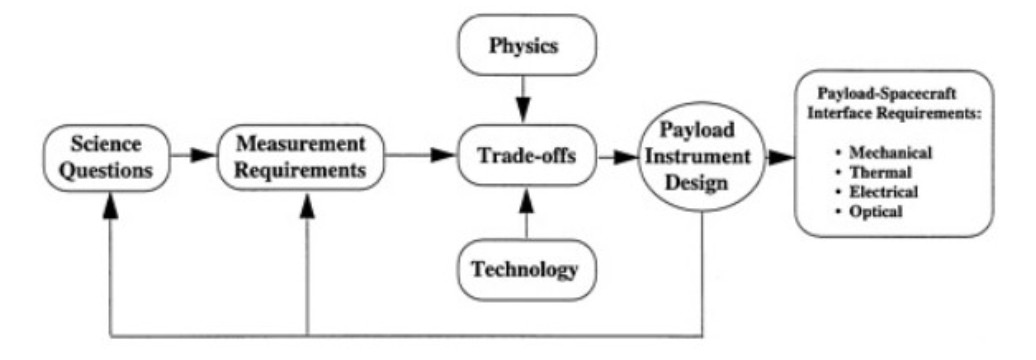
\includegraphics[width=0.8\textwidth]{figures/3.16.jpg}
    \caption{\protect\href{https://nap.nationalacademies.org/read/9819/chapter/5\#23}
    {Le processus de conception de la charge utile génère des exigences pour son intégration. Image courtoisie de NASA et NAP.}}
    \label{fig:communication2}
\end{figure}
\textbf{Définition de l'Architecture de Mission}

\begin{itemize}
    \item Une fois une \textbf{charge utile} identifiée et validée en respectant toutes les contraintes, la conception de l'architecture de mission peut commencer.
    \item Nous avons abordé les solutions pour les différents \textbf{composants de la mission}.
    \item Concernant le \textbf{concept des opérations}, nous nous concentrerons sur :
    \begin{itemize}
        \item La \textbf{durée de vie de la mission}.  
        \item La \textbf{séquence des événements} après l'arrivée du satellite dans l'espace.  
    \end{itemize}
\end{itemize}
\textbf{Spécificités du Kit Artemis}

\begin{itemize}
    \item Le \textbf{kit Artemis CubeSat} n'a pas de \textbf{durée de vie définie} ni de \textbf{concept d’opération spécifique}, car ils dépendent fortement de l’objectif de mission et de la charge utile.  
    \item La mission \textbf{Ke Ao}, une implémentation du kit Artemis CubeSat, a une \textbf{durée opérationnelle d’un an}.  
    \item Le concept d’opération de la mission Ke Ao est défini comme suit :
\end{itemize}

\textbf{Conception du Bus Spatial}

\begin{itemize}
    \item Une fois l’\textbf{architecture de mission} définie, la conception du \textbf{bus spatial} peut être réalisée en fonction de la charge utile, tout en tenant compte des opérations et des composants de la mission.  
    \item Quel que soit le type de charge utile, la conception du bus spatial doit satisfaire aux exigences de :
    \begin{itemize}
        \item \textbf{Données} générées par la charge utile.  
        \item \textbf{Taille}, \textbf{poids} et \textbf{puissance} (\textbf{SWaP}).  
    \end{itemize}
    \item Pour une charge utile d’observation, l’interface entre la charge utile et le bus spatial repose sur plusieurs exigences :
    \begin{itemize}
        \item \textbf{Mécaniques}.  
        \item \textbf{Thermiques}.  
        \item \textbf{Électriques}.  
        \item \textbf{Spécifiques au sujet observé}.  
    \end{itemize}
\end{itemize}
\begin{table}[h]
    \centering
    \renewcommand{\arraystretch}{1.2} % Ajuste l'espacement vertical
    \begin{tabular}{|l|l|l|l|}
        \hline
        \textbf{Mécanique} & \textbf{Thermique} & \textbf{Électrique} & \textbf{Spécifique au sujet} \\
        \hline
        Taille (Structures et Lanceur) & Flux thermique conduit et rayonné vers/depuis la charge utile (Thermique) & Exigences de puissance (Énergie) & Orientation des capteurs et champs de vision dégagés (Structures) \\
        \hline
        Masse (Structures et Lanceur) & Gradients thermiques et distorsion de la plaque de base (Thermique et Structures) & Débit de données en sortie et stockage (CDH) & Stabilité du pointage, agilité (ADCS) \\
        \hline
        Moments d'inertie (Structures) &  & Commande, contrôle et télémétrie (Communications et Segment Sol) &  \\
        \hline
        Contamination : particules, dégazage (Tests environnementaux) &  & Interférences électromagnétiques (Tests environnementaux) & Niveau d'autonomie et opérations (Architecture de mission) \\
        \hline
        Charges de lancement (Tests environnementaux et Lanceur) &  &  &  \\
        \hline
        Perturbations (Tests environnementaux et Orbite) &  &  &  \\
        \hline
    \end{tabular}
    \caption{Contraintes mécaniques, thermiques, électriques et spécifiques au sujet}
    \label{tab:mechanical_constraints}
\end{table}
\textbf{Impact de la Charge Utile sur les Sous-Systèmes du Bus Spatial}
Chaque sous-système du bus spatial et composant périphérique de la mission est mentionné au moins une fois dans le tableau des exigences d'intégration de la charge utile. Les sous-systèmes du bus spatial sont influencés par la charge utile de la manière suivante :
\begin{itemize}
    \item \textbf{Structures} : 
    la charge utile peut nécessiter :
    \begin{itemize}
        \item Une certaine \textbf{orientation} dans le cadre du vaisseau spatial (par exemple, orientée vers l'extérieur du centre du vaisseau).  
        \item Un \textbf{champ de vision dégagé} vers l’environnement spatial (notamment pour les systèmes optiques).  
        \item L’\textbf{intégration de dimensions et de masses spécifiques}.  
        \item Des \textbf{mécanismes actifs} ou des \textbf{éléments déployables} (comme un bras extensible).  
    \end{itemize}
		\begin{figure}
    			\centering
    			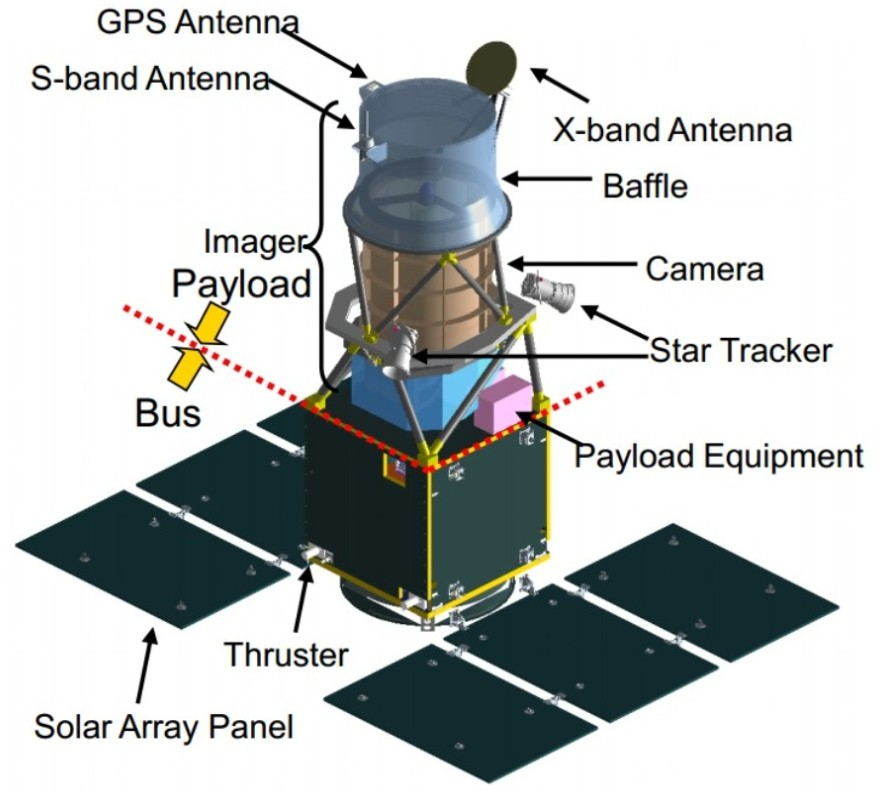
\includegraphics[width=0.8\textwidth]{figures/3.17.jpg}
    			\caption{ASNARO-1 Satellite has many components that have unobstructed views or access to the space environment, like the star tracker, 					camera, imager, and antennas” Image Courtesy of NEC.}
    			\label{fig:communication2}
			\end{figure}
    	\begin{figure}[H]
    		\centering
    		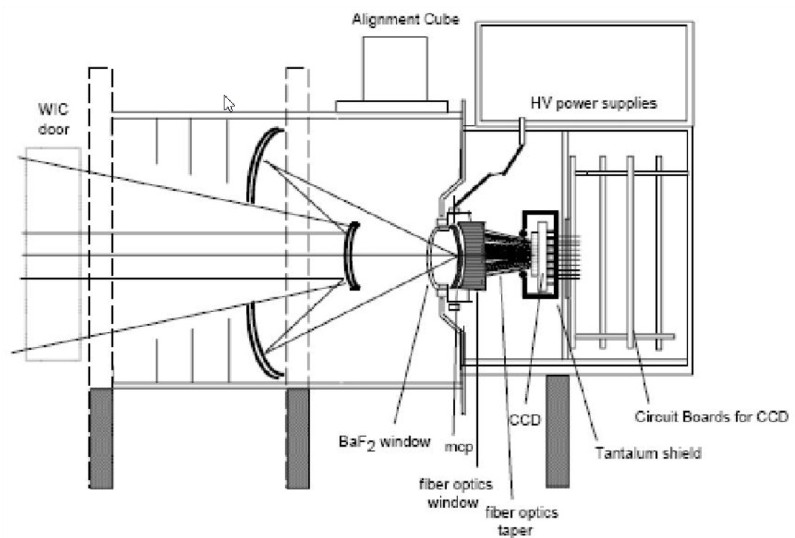
\includegraphics[width=0.8\textwidth]{figures/3.18.jpg}
    		\caption{Schematic view of the Wideband Imaging Camera (WIC) instrument, showing the placement of the power supply with respect to the 							instrument. Image courtesy of UCB/SSL.}
    		\label{fig:communication2}
	\end{figure}
    \item \textbf{Puissance} : la charge utile peut nécessiter :
    \begin{itemize}
        \item Une \textbf{puissance moyenne orbitale} et une \textbf{puissance de crête} adaptées à la distribution électrique (\textit{câblage, carte 					mère et contrôle des cartes filles}).  
        \item Une quantité spécifique de \textbf{puissance générée et/ou stockée} (\textit{taille des panneaux solaires et des batteries}).  
        \item Une \textbf{conversion de tension} et des \textbf{limites de tension} (\textit{conception des circuits imprimés}).  
        \item Une \textbf{régulation du courant} et des \textbf{limites de courant} (\textit{conception des circuits imprimés}).  
    \end{itemize}
    \item \textbf{Commande et Traitement des Données} : la charge utile peut nécessiter :
    \begin{itemize}
        \item Une \textbf{vitesse de traitement} suffisante (\textit{processeurs embarqués : CPU, GPU, RAM}).  
        \item Une \textbf{capacité de stockage des données} adéquate (\textit{mémoire embarquée : carte SD, disque dur}).  
        \item Un \textbf{format de données spécifique} (\textit{image, spectres de fréquence}).  
        \item Une \textbf{bande passante} suffisante pour le transfert des données (\textit{algorithmes pour éviter la surcharge mémoire}).  
        \item Une \textbf{résolution des données} adaptée (\textit{nombre de chiffres significatifs à conserver dans les mesures}).  
    \end{itemize}

    \item \textbf{Communications} : la charge utile peut nécessiter :
    \begin{itemize}
        \item Un \textbf{bilan de liaison} fiable avec une marge suffisante (\textit{transmission bidirectionnelle stable}).  
        \item Un \textbf{débit de liaison montante} adapté (\textit{modes critiques de fonctionnement durant la mission}).  
        \item Un \textbf{débit de télémétrie en liaison descendante} suffisant (\textit{éviter la saturation de la mémoire embarquée}).  
    \end{itemize}
    \item \textbf{Détermination, Contrôle d'Attitude et Navigation} : la charge utile peut nécessiter :
    \begin{itemize}
        \item Une \textbf{précision et exactitude} dans le pointage, le pivotement ou le suivi (\textit{systèmes de contrôle du moment angulaire}).  
        \item Une \textbf{résolution spécifique} dans l'estimation de l'attitude ou de la position (\textit{algorithmes d'estimation, capteurs}).  
    \end{itemize}
\end{itemize}
\textbf{Lectures Suggérées :}  
\textit{\href{https://trs.jpl.nasa.gov/bitstream/handle/2014/41915/11-0422.pdf?sequence=1}
{Instrument Pointing Capabilities: Past, Present, and Future}}

\begin{figure}[H]
    	\centering
    	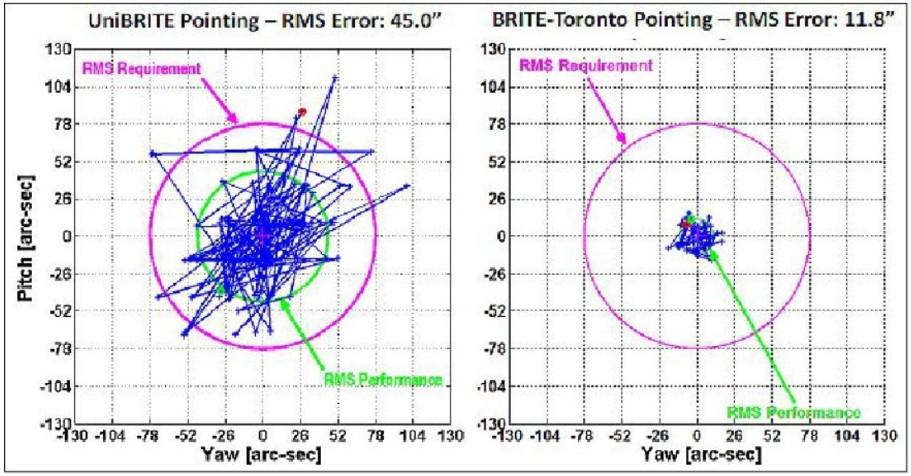
\includegraphics[width=0.8\textwidth]{figures/3.19.jpg}
    	\caption{The primary mission objective of BRITE Constellation is to provide milli-magnitude differential photometry of bright stars. On-orbit fine pointing performance of UniBRITE spacecraft (left) and BRITE-Toronto spacecraft (right)}
    	\label{fig:communication2}
\end{figure}
\textbf{Impact de la Charge Utile sur le Sous-Système Thermique}
\begin{itemize}
    \item \textbf{Thermique} : la charge utile peut nécessiter :
    \begin{itemize}
        \item Une \textbf{plage de fonctionnement thermique spécifique} (\textit{les systèmes optiques, par exemple, préfèrent être maintenus à basse température}).  
        \item Une \textbf{stabilité structurelle face aux variations de température} :
        \begin{itemize}
            \item Utilisation de \textbf{matériaux résistants à la dilatation thermique}.  
            \item Maintien d’une \textbf{température stable} pour éviter les déformations mécaniques.  
        \end{itemize}
    \end{itemize}
\end{itemize}
\begin{figure}[H]
    	\centering
    	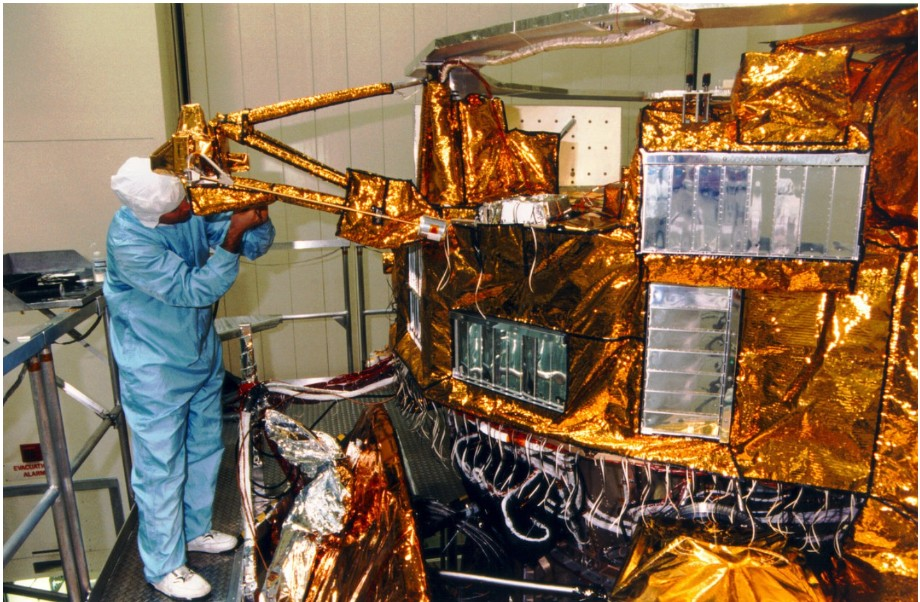
\includegraphics[width=0.8\textwidth]{figures/3.20.jpg}
    	\caption{A unique combination of meticulous old-world skills and high-tech materials produced the finely sewn, super-strong, and extremely lightweight thermal blankets that protected Cassini from the extreme hot and cold of deep space. Image courtesy of NASA.}
    	\label{fig:communication2}
\end{figure}
